% !TEX root = ../../thesis.tex
\chapter{Diophantine Equations\label{ch:dioeq}}
\pagestyle{fancy}

% Historical Context
\section{Historical Context}

Number Theory is among the oldest fields of Mathematics. This fact is owed mostly to ancient culture's study of Diophantine equations, named in reference to the 3rd century mathematician Diophantus of Alexandria who systematically studied these equations.


\begin{dfn}[Diophantine Equation]
A Diophantine equation is an equation of the form $f(x_1,\ldots,x_n)= 0$, where $f(x_1,\ldots,x_n) \in \Z[x_1,\ldots,x_n]$, with the only allowed solutions are integers (or more generally rational numbers).
\end{dfn}


Such equations arose naturally for ancient cultures, especially in the context of division of resources for allocation. For example, Diophantine equations can be found in the Rhind Papyrus of Egypt, the Chinese Jiuzhang, the Babylonian Plimpton, ancient Indian, Islamic, and Greek texts, etc. As an explicit example, consider Problem~17 of the Jiuzhang found in \cite{vogel68}: ``the price of 1~acre of good land is 300 pieces of gold; the price of 7~acres of bad land is 500. One has purchased altogether 100~acres; the price was 10,000. How much good land was bought and how much bad.'' This gives a system of equations
	\[
	\begin{aligned}
	x + y&= 100 \\
	300x + \dfrac{500}{7}\,y&= 10,000,
	\end{aligned}
	\]
which of course is equivalent to the system of Diophantine equations
	\[
	\begin{aligned}
	x + y&= 100 \\
	2100x + 500y&= 70,000,
	\end{aligned}
	\]
yielding solutions $x= 25/2$ and $y= 175/2$. For more on this history with examples see \cite{katz09}. Diophantine equations were also studied extensively in European mathematics, especially in the work of Euler, Gauss, Legendre, Dirichlet, Kummer, Sylvester, Weierstrass, Hermite, Eisenstein, Fermat, Kronecker, Dedekind, Germain, Poincar\'e, etc. The development of tools to study these equations led to enormous growth in Algebraic Geometry, Complex Analysis, Algebraic and Analytic Number Theory, Algebra, etc. 


Of course, a Diophantine equation need not have any solutions. For example, the equation $x^2 + y^2= 3$ has no rational solutions. A fortiori, there are no rational solutions to this equation. To see this, suppose there were rational numbers satisfying the equation. Clearing denominators, we would then have integers $X,Y,Z$ such that $X^2 + Y^2= 3Z^2$. Without loss of generality, by cancelling common factors, we assume that $\gcd(X,Y,Z)= 1$. Examining the equation modulo 3, we see that 3 divides $X^2 + Y^2$, but as the only possible square values modulo 3 are 0 and 1, this implies that $X^2$ and $Y^2$, and hence $X$ and $Y$, are divisible by 3. But this implies that $Z^2$, and hence $Z$, is divisible by 3, a contradiction. Such `modularity' conditions can be used to prove the nonexistence of rational solutions to equations such as $y^2= 3x^2 + 2$, $3y= x^2 - 5$, $x^5 + y^5 + z^5= 2021$, etc. The technique here can be generally summarized as follows: a solution to a Diophantine equation naturally leads to a real solution and a solution modulo every (prime) modulus. Showing that a certain modulus has no solutions proves the nonexistence of integer solutions. 


However, the converse is not necessarily true. This naturally leads to a discussion of the local-to-global (or Hasse) principle, which essentially is that a Diophantine equation over $\Q$ has rational solutions ``if and only if'' it has a real solution and a solution mod-$n$ for $n \geq 2$. Using the Chinese Remainder Theorem, this is equivalent to the statement that a Diophantine equation over $\Q$ has rational solutions ``if and only if'' it has a real solution and a solution modulo $p^k$ for all $k$, i.e. a solution in $\Q_p$ for all primes $p$.\footnote{Note, we are being a bit loose and flippant with the details and technicalities here.} Of course, this ``if and only if'' is not an equivalence at all. Selmer gave the example of $3x^3 + 4y^3 + 5z^3= 0$ in \cite{selmer51}, which has only the trivial solution over $\Q$ but possesses a nonzero real solution and a solution in $\Q_p$ for every $p$, see \cite{conradselmer}. The famous theorem of Hasse-Minkowski states that the local-to-global principle holds for quadratic forms. 


\begin{thm}[Hasse-Minkowski]
A homogeneous quadratic equation in several variables is solvable by rational numbers (not all zero) if and only if it is solvable in $\Q_p$ for all $p$, including $p= \infty$ (the case of $p= \infty$ is the case of $\R$). 
\end{thm}


David Hilbert asked if there was an algorithm to determine if a given Diophantine equation has a solution. This was Hilbert's tenth problem of twenty-three proposed at the 1900 International Congress of Mathematicians in Paris. Matiyasevich, Putnam, and Robinson answered this question in the negative, see \cite{matiyasevich93}. Of course, one can ask a ``Hilbert tenth problem'' question for equations over rings other than $\Z$. This is a deep topic with connections to many different areas of Mathematics and is still an active area of research with several papers on the topic being released just this year, e.g. \cite{hilbert1}, \cite{hilbert2}, or \cite{hilbert3}. For more on this topic, see \cite{poonenhilbert}. 


        \begin{table}[!ht]
        \centering
        \caption{A table from \cite{poonenhilbert} indicating whether Hilbert's tenth Problem holds for various fields of increasing arithmetic complexity (measured by $\Gal(\ov{K}/K)$).\label{tab:hilbert10}}
        \begin{tabular}{|c|c|c}  \cline{1-2}
        Ring & Hilbert's 10\textsuperscript{th} & \hspace{1cm} \llap{\tikz[remember picture]\node (top node){};\hspace*{1em}} \\ \cline{1-2}
        $\C$ & \cmark \\
        $\R$ & \cmark \\
        $\F_q$ & \cmark \\
        $p$-adic fields & \cmark \\
        $\F_q(\!(t)\!)$ & ? \\
        Number Fields & ? \\
        $\Q$ & ? \\
        Global Function Fields & \xmark \\
        $\F_q(t)$ & \xmark \\
        $\C(t)$ & ? \\
        $\C(t_1,\ldots,t_n)$ & \xmark \\
        $\R(t)$ & \xmark \\
        $\cO_K$ & $\approx$? \\
        $\Z$ & \xmark & \hspace{1cm} \llap{\tikz[remember picture]\node (bottom node){};\hspace*{1em}} \\ \cline{1-2}
        \end{tabular}
        \end{table}





% Linear Diophantine Equations
\section{Linear Diophantine Equations \label{sec:linearequations}}

For Diophantine equations in one variable, it is a simple matter to determine all the integer (or rational) solutions to the equation using the Rational Roots Theorem.


\begin{thm}[Rational Roots Theorem] \label{thm:rationalroot}
If $f(x)= a_nx^n + a_{n-1}x^{n-1} + \cdots + a_1x + a_0 \in \Q[x]$, then the equation $f(x)= 0$ has a rational solution $x= p/q$ only if $p \mid a_0$ and $q \mid a_n$. 
\end{thm}


Theorem~\ref{thm:rationalroot} gives a finite list of possible rational roots (and hence possible integer solutions) which one then need only test. The case of linear Diophantine equations in $n$ variables $x_1, \ldots, x_n$ is also equally simple to solve. Suppose we had an equation of the form $a_1x_1 + \cdots + a_nx_n= d$, where $a_i, d \in \Q$. Clearing denominators, we obtain an equation $a_1'x_1 + \cdots + a_n'x_n= d'$, where $a_i', d' \in \Z$. This equation has integer solutions if and only if $\gcd(a_1',\ldots,a_n')$ divides $d'$, see \cite[Thm.~1.15]{nathanson00}. Clearly, if there are integer solutions, there are rational solutions. Therefore, Diophantine equations in $n$ variables have a rational solution if and only if there is  an integer solution. Furthermore, it is equally simple to solve linear congruences (though a somewhat more difficult task for higher congruences) using the Chinese Remainder Theorem, the theory of primitive roots, and Quadratic Reciprocity, though we will not discuss this here, see Chapter~2 and 3 of \cite{nathanson00}. 





% Quadratic Diophantine Equations
\section{Quadratic Diophantine Equations\label{sec:quaddioeq}}

The study of quadratic Diophantine equations is really the study of conics. Of course, we shall assume our conics are nondegenerate (which are not difficult to handle). Consider a conic given by a quadratic Diophantine equation
	\[
	f(x,y):= a + bx + cy + dx^2 + exy + fy^2= 0.
	\]
Note that the Hasse Principle does apply for conics. We have already seen in the example of the circle $x^2 + y^2= 3$ that a conic need not possess any rational points whatsoever. However when the conic does have a rational point, there is an easy way of finding all rational points on the curve. We will examine this in the simple case of $x^2 + y^2= 1$. We will need a theorem of B\'ezout:

\begin{thm}[B\'ezout] \label{thm:bezout}
Let $F, G \in K[x,y,z]$ be homogeneous curves of degree $m,n$, respectively. Then if $F(\ov{K}) \cap G(\ov{K})$ is nonempty and $F,G$ do not share a homogeneous polynomial of positive degree as a factor, then $F$ and $G$ intersect at precisely $nm$ points in projective space. 
\end{thm} 

	\begin{figure}[!ht]
	\centering
	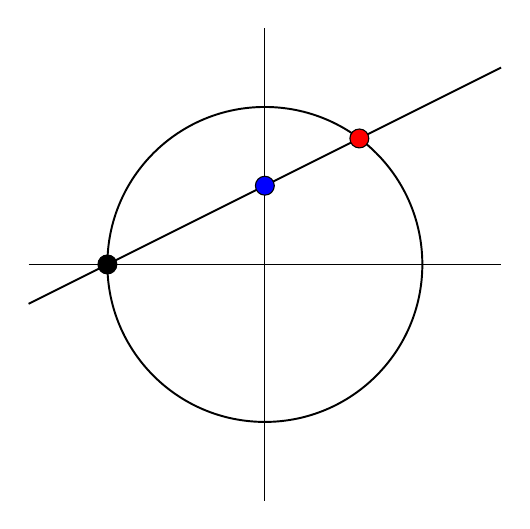
\begin{tikzpicture}[scale=2]
	\draw (-1.5,0) -- (1.5,0);
	\draw (0,-1.5) -- (0,1.5);

	\draw[line width=0.7] (-1.5,-0.25) -- (1.5,1.25);
	\draw[line width=0.7] (0,0) circle (1);
	
	\draw[fill=black] (-1,0) circle (0.06);
	\draw[fill=blue] (0,0.5) circle (0.06);
	\draw[fill=red] (0.6,0.8) circle (0.06);
	\end{tikzpicture}
	\caption{Finding the rational points on the circle $x^2 + y^2= 1$.\label{fig:circle}}
	\end{figure}

The circle $x^2 + y^2= 1$ has a rational point $(-1,0)$ (the black point in Figure~\ref{fig:circle}). Drawing the line through $(-1,0)$ and a point $(0,q)$, where $q \in \Q$, this line intersects the circle at another point distinct from $(-1,0)$ (shown in red in Figure~\ref{fig:circle}) by Theorem~\ref{thm:bezout}. Moreover because the point $(-1,0)$ is rational, this second point of intersection is rational. Conversely, choose a rational point distinct from $(-1,0)$ on the circle. Drawing the line through this point and $(-1,0)$, we see this line must intersect $x= 0$ at a rational point. With a bit of algebra, we can see that the set of rational points on this circle, $\cC(\Q)$, is the following set:
	\[
	\cC(\Q)= \{ (-1,0) \} \cup \left\{ \left(\dfrac{1-t^2}{1+t^2}, \dfrac{2t}{1+t^2} \right) \colon t \in \Q \right\}.
	\] 
The point $(-1,0)$ corresponds to a vertical line through $(-1,0)$ which intersects the conic at the point at infinity in projective space. The vertical line through $(-1,0)$ also intersects the line $x= 0$ at the point at infinity. It is then simple to see that $\cC(\Q)$ is isomorphic to the projective line $\P^1(\Q)$. 


There is nothing special about the case of the circle. We could have used this approach for any conic with a rational point. But of course in the conic case, we are dealing with a curve of degree 2 so that the genus is 0 by the following well known formula:
	\[
	g= \dfrac{(d - 1)(d - 2)}{2}.
	\]
In fact, a more general result is true.


\begin{thm}[{\cite[Thm.~A.4.2.7]{hindrysilverman00}}] \label{thm:genusdegree}
Let $\cC$ be a projective plane curve of degree $d$ with only ordinary singularities. Then its genus is given by
	\[
	g= \dfrac{(d - 1)(d - 2)}{2} - \sum_{P \in S} \dfrac{m_P(m_P - 1)}{2},
	\]
where $S$ is the set of singular points and $m_P$ is the multiplicity of $\cC$ at $P$.
\end{thm}

	
The converse is true in a sense as well. Suppose $\cC$ is a smooth projective curve of genus 0 over a field $F$. Let $K_\cC$ be a canonical divisor over $F$ associated to $\cC$. Using the Riemann-Roch theorem, it is simple to see that $-K_\cC$ is a very ample divisor of degree 2 over $F$. Then the dimension of the associated embedding is $\ell(-K_C)= 3$. Therefore, $C$ can be embedded into $\P^2$ as a smooth curve of degree 2 defined over $F$, i.e. a conic over $F$. Then the above `circle method' applies whenever this conic has a $F$-rational point. Thus, we have the following description of quadratic Diophantine equations:


\begin{thm} \label{thm:genus0case}
Let $C$ be a smooth projective curve of genus 0 defined over a field $k$. Then
\leavevmode\vspace{-2em}
	\begin{enumerate}[(i)]
	\item the curve $\cC$ is isomorphic over $F$ to a conic in $\P^2$.\leavevmode\vspace{-2em}
	\item the curve is isomorphic to $\P^1$ over $F$ if and only if it possess a $F$-rational point.
	\end{enumerate}
\end{thm}





% Higher Diophantine Equations
\section{Higher Diophantine Equations\label{sec:highdioeq}}

For Diophantine equations given by smooth functions of many variables with sufficiently high degree, we can see from Theorem~\ref{thm:genusdegree} that the corresponding curves will have genus $g > 1$. We have already seen that rational points on linear Diophantine equations arise from divisibility conditions `alone.' In the case of quadratic Diophantine equations, rational solutions arise from the fact (assuming $\cC(\Q) \neq \emptyset$) that $\cC(\Q) \cong \P^1(\Q)$. As a `moral argument,' one may summarize this as Diophantine equations `have no business' having rational solutions at all unless there is a `good reason.' For higher degree Diophantine equations, one might then expect them to have no rational solutions at all, or at most finitely many. Indeed, this was Mordell's conjecture in 1922 (or the Mordell-Lang Conjecture). This conjecture was later proved by Gerd Faltings, earning him the Fields Medal.


\begin{thm}[{Faltings, \cite{faltings84}}] \label{thm:faltings}
Let $\cC/K$ be a smooth, projective, and geometrically irreducible\footnote{The curve stays irreducible after extending to the algebraic closure.} curve of genus $g \geq 2$ over a number field $K$. Then the set $\cC(K)$ is finite. 
\end{thm}


For more on this amazing theorem, see \cite{snowdenbhatt16}. Though Falting's theorem proves there are at most finitely many rational solutions on `most' higher degree Diophantine equations, it does not say how to actually compute this finite set. Faltings used Arakelov methods for his proof of Theorem~\ref{thm:faltings}. There are other proofs of Faltings' theorem by Vojta (see \cite{vojta91}) using Diophantine approximation, a proof of Bombieri (see \cite{bombieri90}) altering Vojta's approach, and a proof of Lawrence-Vankatesh (see \cite{lawrencevankatesh20}) using $p$-adic period maps. Perhaps more importantly, there is a method of Chabauty, using Coleman integration and an adaptation of the $p$-adic method of Skolem, that proves if the Jacobian of $\cC$ satisfies $J(\cC) < g$, then $\cC(K)$ is finite. Because computing all the $K$-rational points on higher genus curves is a necessity in many torsion classifications, we will give a small flavor of the approach following the description of Poonen, see \cite{poonen20}. 


Let $\cC/K$ be a smooth projective, geometrically integral curve of genus $g \geq 2$, and let $J$ be the Jacobian of $\cC$---an abelian variety of dimension $g$ over $K$. Let $K/\Q$ be a number field, and $\fp$ a prime above $p$ over which $\cC$ has good reduction. Suppose we had a $K$-rational point $\cO \in \cC(K)$. Then we have an Abel-Jacobi embedding $\iota: \cC \hookrightarrow J$ given by $P \mapsto [P - \cO]$. If we do not have a $K$-rational point, we can always scale $P$ to find an effective divisor for an equally good substitute. The idea is to compute $J(\cC)$, and then determine which of the $K$-rational points in the Jacobian actually lie on $\cC$. 


	\begin{figure}[!ht]
	\centering
	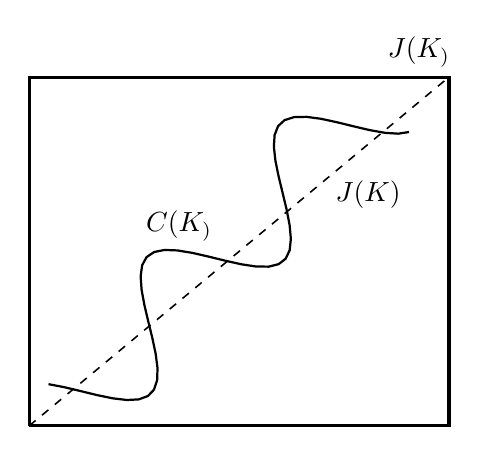
\begin{tikzpicture}
	\begin{axis}[
	hide axis,
	xmin=-3, xmax=6,
	ymin= -2, ymax= 7
	]
	\draw[line width=0.04cm] (-2,-1) -- (5,-1) -- (5,6) -- (-2,6) -- (-2,-1);
	\draw[line width= 0.02cm,dashed] (-2,-1) -- (5,6);
	\addplot[domain=-0.1*pi:2.2*pi, samples=50, black,thick,rotate=45] ({\x+0.5},{-sin(2*\x r)-3});
	\node at (0.5,3) {$C(K_\fp)$};
	\node at (4.5,6.5) {$J(K_\fp)$};
	\node at (3.65,3.65) {$J(K)$};
	\end{axis}
	\end{tikzpicture}
	\caption{A graphical representation of the embedding $C(K_\fp)$ into $J(K_\fp)$.\label{fig:chab}}
	\end{figure}


Because we have more structure after completion, we will work with the $p$-adic Lie group $K_\fp$. Then the set $\cC(K_\fp)$ is the set of local points on the curve $\cC$ and is an analytic submanifold of the Lie algebra of $J(K_\fp)$. Because the $K$-rational points of $\cC$ lie in both the Mordell-Weil group of $\cC$ and $\cC(K_\fp)$, what we want to find is the intersection of the Mordell-Weil group of $\cC$ (the dotted line in Figure~\ref{fig:chab}) with $\cC(K_\fp)$. The Abel-Jacobi map takes rational points to rational points, so everything is happening inside the ambient Lie group $J(K_\fp)$. So the $K$-rational points are in the intersection of the local points $\cC(K_\fp)$ and the group $J(K)$. We compute this intersection with the hope that this will just be the $K$-rational points with nothing `extra.' Using the formal logarithm map, we base change from $J(K_\fp)$ to the local field obtained by integrating 1-forms $p$-adically. This takes the group law to an addition law in the vector space $K_\fp^g$, where intersections will be simpler to compute. Now assume that $r < g$. There then exists a nonzero functional $\lambda$ vanishing on $\im J(K)$. Now on each residue disk $\lambda$ is represented by a (nonzero) power series in a 1-dimensional space. Therefore, $\lambda$ has at most finitely many zeros on each closed disk in this compact space. But then $\lambda$ pulls back to a nonzero locally analytic function on $\cC(K_\fp)$ vanishing on $\cC(K)$. Therefore, $\cC(K)$ is finite. 


\begin{thm}[{\cite{chabauty41}, \cite[Cor.~4a]{coleman85}, \cite[Thm.~5.3b]{mccallumpoonen12}}]
Let $\cC$ be a smooth, projective, and geometrically integral scheme of dimension 1 over $\spec(\Q)$ with genus $g \geq 2$ over $\Q$, and let $J$ be its Jacobian variety. Let $p$ be a prime number. Suppose that the rank of $J(\Q)$ is smaller than $g$, $p > 2g$, and $\cC$ has good reduction at $p$. Then $\#\cC(\Q) \leq \#\cC(\F_p) + (2g - 2)$.
\end{thm}


Obviously, Jacobians are difficult to work with. Moreover, one has the tedious restriction of $r < g$. The work of Minhyong Kim tries to replace Jacobians instead with homology groups of $\cC$, developing a non-abelian Chabauty method which is much more powerful than ordinary Chabauty. We will not discuss this farther. For more on this topic, see the notes from the 2020 Arizona Winter School at \cite{arizona}. Finally, we remark there is a much more `high brow' approach to much of what we have discussed here in terms of general results from Algebraic Number Theory and Algebraic Geometry, see \cite{hindrysilverman00} and \cite{poonen17}.





% Curves of Genus g = 1
\section{Curves of Genus $g= 1$\label{sec:genus1}}

% Elliptic Curves
\subsection{Elliptic Curves\label{sec:g1ec}}

We know (modulo technicalities) that curves of genus $g= 0$ have infinitely many $K$-rational points; moreover, we know how to find them. For curves of genus $g > 1$, we know there are at most finitely many $K$-rational solutions---though finding an effective way to compute this set (especially in higher genus) is still a difficult open problem. This leaves the case of genus $g= 1$, which is the case of elliptic curves. In a sense, this is the most interesting case in that the set of $K$-rational points can be empty, finite, or infinite. 


% Motivating Examples
\section{Motivating Examples\label{sec:motivex}}

We will now see a few scenarios in which elliptic (and hyperelliptic) curve naturally arise that highlight why one would be interested in elliptic curves as well as their connection to other areas in Mathematics. We begin with the classic cannonball arrangement.


% Cannonball
\begin{ex}[{The Cannon Ball Problem, \cite{washington03}}]
Suppose one has a square pyramid of cannonballs. No longer stable, the pile collapses and the balls scatter. For what size pyramid can these balls now instead be arranged into a square grid? It is clear this possible for the trivial pile with 0 cannon balls, as well as a pile with 1 cannon ball. Obviously, there are pile sizes that do not have this property. For instance, if the pile is 2 layers high, then there are 5 total cannon balls, which clearly cannot be arranged into a square grid as 5 is not a perfect square. 

If the pyramid began with $x$ layers, then the total number of cannon balls is
	\[
	1^2 + 2^2 + \cdots + x^2= \dfrac{x(x + 1)(2x + 1)}{6}.
	\]
For these cannonballs to be arranged into a square grid, their total must be a perfect square; that is, there is a $y \in \Q$ with
	\begin{equation} \label{eqn:initialec}
	y^2= \dfrac{x(x + 1)(2x + 1)}{6}.
	\end{equation}
A method of Diophantus finds us more points: we know the points $(0,0)$ and $(1,1)$ are on this curve. The line through these points is $y= x$. Intersecting this line with $y^2= (x(x + 1)(2x + 1))/6$, we obtain the solution $(1/2,1/2)$. Clearly, if $(x,y)$ is a solution to the equation, then so is $(x,-y)$. Then we have an additional solution $(1/2,-1/2)$. We can repeat this procedure using the points $(1/2,-1/2)$ and $(1,1)$. This gives a solution of $(24,70)$. One can repeat this method of Diophantus to produce more rational solutions---though none of them will be integer valued. 

What is happening here is addition of points on an elliptic curve. After multiplication by 6 in \eqref{eqn:initialec} and making a substitution of $Y= 72y$ and $X= 12x + 6$, we see that the curve in \eqref{eqn:initialec} is isomorphic to the elliptic curve $E: Y= X^3 - 36X$ with Cremona label \fssht{}. We have $E \cong \Z \oplus \Z/2\Z \oplus \Z/2\Z$. By a theorem of Siegel, c.f. Theorem~\ref{thm:siegel}, there are only finitely many integer valued points on $E$. In this case, the only integral points are $(0,0), (1,\pm1), (24, \pm 70)$.
\end{ex}


% Fermat's Last Theorem
\begin{ex}[Fermat's Last Theorem]
In a marginal note in Fermat's copy of the {\itshape Arithmetica}, Pierre de Fermat noted, 
	\begin{quote}
	Cubum autem in duos cubos, aut quadratoquadratum in duos quadratoquadratos \& generaliter nullam in infinitum ultra quadratum potestatem in duos eiusdem nominis fas est dividere cuius rei demonstrationem mirabilem sane detexi. Hanc marginis exiguitas non caperet.
	\end{quote}
That is, he has a truly marvelous proof that $x^n + y^n= z^n$ had no nontrivial solutions for $n > 2$, but the margins were too narrow to contain it. In fact, Fermat's copy of the Arithmetica contained many unproven marginal notes, which mathematicians took upon themselves to prove (or in some cases disprove). The problem stated above was the last of these marginal notes to be dealt with and became known as Fermat's Last Theorem (though Fermat's Last Conjecture would have been more appropriate). It would take 329 years for someone to prove this statement, although many tried. For a history of this problem, see \cite{singh12} or \cite{ribet95}. Fermat's Last Theorem was ultimately proven by Wiles and Taylor-Wiles. In fact, Wiles did not prove Fermat's Last Theorem directly. Instead, Wiles proved a statement about elliptic curves. 

In 1984, Gerhard Frey assumed that there was a nontrivial solution $(a,b,c)$ for exponent $p > 2$.\footnote{To prove Fermat's Last Theorem, it suffices to prove it for prime $p > 2$.} He then conjectured that the (semistable) elliptic curve, now called the `Frey curve',
	\[
	y^2= x ( x - a^p)(x + b^p)
	\]
would not be modular, although he was unable to prove this, see \cite{frey86}. This gap became known as the $\epsilon$-conjecture. Serre gave a near proof which was completed in 1986 by Ribet \cite{ribet90}. Using ideas of Iwasawa Theory, modular forms, and new techniques in Euler systems developed by Flach and Kolyvagin, Wiles gave a near proof of Fermat's Last Theorem in 1993 by proving that all semistable elliptic curves are modular. The proof contained a small gap that was filled in the next year by Wiles and Richard Taylor, a former Ph.D. student of Wiles, see \cite{wiles95} and \cite{taylorwiles95}.

This was enough to establish Fermat's Last Theorem. Later work of Breuil, Conrad, Diamond, Taylor in \cite{conraddiamondtaylor99} and \cite{breuilconraddiamondtaylor01} would fully prove the Taniyama-Shimura conjecture (now known as the Modularity Theorem) that all rational elliptic curves are modular. There exist other generalizations to Fermat's Last Theorem: the Generalized Fermat Equation (or Beal conjecture), Inverse Fermat Equation, etc. 
\end{ex}


% Congruent Number Problem
\begin{ex}[Congruent Number Problem]
What natural numbers $n$ are the areas of rational right triangles, i.e. right triangles whose sides are rational. We call such integers $n$ congruent. This is equivalent to a rational triplet $(x,y,z)$ with
	\[
	x^2 + y^2= z^2 \quad \text{ and } \quad n= \dfrac{xy}{2}.
	\]
The history of this problem dates back to at least 972~AD, see \cite{dickson71}. Clearly, $6$ is congruent because $3^2 + 4^2= 5^2$ and $6= \frac{3(4)}{2}$. However, restricting to integer sides is not sufficient. Observe that the triangle with sides $3/2$, $20/3$, and $41/6$ has area 5. Furthermore, 157 is a congruent number, as Zagier proved in \cite{zagier90} with the following example:
	\[
	\begin{aligned}
	x&= \dfrac{411340519227716149383203}{21666555693714761309610} \\
	y&= \dfrac{6803298487826435051217540}{411340519227716149383203} \\
	z&= \dfrac{224403517704336969924557513090674863160948472041}{8912332268928859588025535178967163570016480830}.
	\end{aligned}
	\]
It is not known which numbers in general are congruent, and given an integer it is not always a simple task to tell if $n$ is congruent or not. Certainly, if $n$ is congruent, then so too is $m^2n$ for all natural numbers $m$. Fermat showed that 1 was not a congruent number using his method of infinite descent. A vast generalization of this type of argument is used in the proof of the Mordell-Weil Theorem. 

Now suppose that $n$ is a congruent number, i.e. there are $(X,Y,Z)$ with $X^2 + Y^2= Z^2$ and $XY= 2n$. Setting $x:= (Z/2)^2$ and $y:= Z(X - Y)(X + Y)/8$, there is a point on the elliptic curve $E_n: y^2= x^3 - n^2x$. Note that $E_n$ is a twist by $n$ of the elliptic curve $y^2= x^3 - x$, which is the elliptic curve with Cremona label \ttat{}. Furthermore, given a rational point $(x,y) \in E_n$, we can define
	\[
	X:= \left| \dfrac{(x - n)(x + n)}{y} \right|, \quad Y:= 2n \left| \dfrac{x}{y} \right|, \quad Z:= \left| \dfrac{x^2 + n^2}{y} \right|.
	\]
It is routine to verify that $X^2 + Y^2= Z^2$ and that $2n= XY$, so that $n$ is congruent. Therefore, finding congruent numbers is equivalent to finding elliptic curves $E_n$ with rank $r > 0$. While many congruent numbers are known, it is still an open problem to determine which integers $n$ are congruent. For more on this problem, see \cite{koblitz93}.
\end{ex}


% Number Theory Example
\begin{ex}[A Diophantine Equation]
What are the integer solutions to $y^2= x^3 - 2$? One can `easily' find the solutions $(3, \pm 5)$, but are these all the solutions? We choose instead to work over the UFD $\Z[\sqrt{-2}]$ in order to make use of the `extra factorization' it has available. Then over $\Z[\sqrt{-2}]$, we have the factorization 
	\[
	x^3= y^2 + 2= (y + \sqrt{-2}) (y - \sqrt{-2}). 
	\]
Writing $x=u_1 \pi_1^{e_1}\cdots \pi_r^{e_r}$, where each $\pi_i$ is irreducible, $e_i \geq 1$, and $\pi_i \neq \pm \pi_j$ for $i \neq j$, we then have
	\[
	u_1^3 \pi_1^{3e_1}\cdots \pi_r^{3e_r}=(y+\sqrt{-2})(y-\sqrt{-2}). 
	\]
We claim that $y + \sqrt{-2}$ and $y - \sqrt{-2}$ are relatively prime: choose an irreducible dividing both, say $\pi$. Then $\pi \mid \big(( y + \sqrt{-2}) - (y - \sqrt{-2}) \big)= 2\sqrt{-2}= (\sqrt{-2})^3$. Note that $\Z[\sqrt{-2}]^\times=\{\pm 1\}$. By unique factorization in $\Z[\sqrt{-2}]$, up to a unit $u$, we must have $\pi= u\sqrt{-2}$. But the only units in $\Z[\sqrt{-2}]$ are $\{\pm 1\}$. Because $\pi^3= (\sqrt{-2})^3$, we must have $\pi= \sqrt{-2}$. Now as $\pi \mid (y + \sqrt{-2})$, we have $y + \sqrt{-2} = \pi (a + b \sqrt{-2})= \sqrt{-2} (a + b\sqrt{-2})= -2b + a\sqrt{-2}$ for some $a, b \in \Z$. But then as $\pi \mid (y + \sqrt{-2})$, we have $y + \sqrt{-2}= \sqrt{-2}(a + b\sqrt{-2})= -2b + a\sqrt{-2}$ for some $a, b \in \Z$. Therefore, $y= -2b$, which implies $x^3= y^2 + 2= 4b^2+2 \equiv 2 \mod 4$, a contradiction as no cube has residue 2 mod 4. This shows that $y + \sqrt{-2}$ and $y - \sqrt{-2}$ are relatively prime.

Then $\pi_i^{3e_i}$ divides $y + \sqrt{-2}$ or $y-\sqrt{-2}$ (but not both) for each $1 \leq i \leq r$. Then $y+\sqrt{-2}= u \prod_{i \in \mathcal{I}} \pi_i^{3e_i}$ for some $\mathcal{I} \subseteq \{ 1, \ldots, r \}$ and $u \in \Z[\sqrt{-2}]^\times= \{ \pm 1 \}$. This implies 
	\[
	y + \sqrt{-2}= u \prod_{i \in \mathcal{I}} \pi_i^{3e_i}= \prod_{i \in \mathcal{I}} \pi_i^{3e_i}= \left( \prod_{i \in \mathcal{I}} \pi_i^{e_i} \right)^3= (a + b\sqrt{-2} \,)^3
	\]
 for some $a,b \in \Z$. Expanding yields, $y+\sqrt{-2}=(a^3-6ab^2)+(3a^2b-2b^3)\sqrt{-2}$. This forces $y= a^3 - 6ab^2$ and $1= 3a^2b - 2b^3= b(3a^2 - 2b^2)$. Now as $b (3a^2 - 2b^2)= 1$ with $a, b \in \Z$, it must be that $b \in \{\pm 1\}$. If $b= 1$, we have $3a^2 - 2= 1$, which gives $a= \pm 1$. Using $a= \pm 1$ and $b=1$, we have solutions $(3, \pm 5)$. If $b= -1$, then $3a^2(-1)-2(-1)^3=1$, which implies $3a^2=1$, a contradiction to the irrationality of $\sqrt{3}$. Therefore, the only integer solutions to $y^2= x^2 + 3$ are $(3, \pm 5)$. 

This proof is indeed tedious. Moreover, it only proves there are only finitely many integer solutions but says nothing of rational solutions. Worse yet, this approach does not necessarily apply to other quadratic rings. For instance, applying this same argument to $y^2= x^3 - 61$ over the ring $\Z[\sqrt{-61}]$, one would `prove' there are no integer solutions, despite the existence of solutions $(5,\pm 8)$. What fails here is unique factorization in the ring, which will not hold for number fields having class number $h_K \neq 1$. 

How does one cope with loss of unique factorization? Kummer (in approximately 1846) said there should be a further factorization into ``ideal numbers'' in order to recover unique factorization. This led Dedekind to define ideals of a ring. He later gave the correct notion of factorization using (prime) ideals rather than factorization with elements. While elements may/may not factor uniquely in $\cO_K$, the ring of integers of $K$, every ideal of $\cO_K$ factors uniquely as a product of prime ideals. In the case of $y^2= x^3 - 61$, while elements $5$, $8 + \sqrt{-61}$, and $8 - \sqrt{-61}$ may not factor uniquely into irreducibles, the ideals generated by these elements will factor uniquely into a product of prime ideals $\fp, \fq$:
	\[
	(5)= \fp \fq, \quad (8 + \sqrt{-61})= \fp^3, \quad (8 - \sqrt{-61})= \fq^3. 
	\]
One can avoid all of this by appealing to the theory of elliptic curves. The curve $y^2= x^3 - 2$ is the elliptic curve with Cremona label \ostevo{} and is isomorphic to $\Z$. Hence, there are infinitely many rational solutions. By Siegel's theorem, there are only finitely many integer solutions. Indeed, there are precisely two---namely $(3 \pm 5)$. 
\end{ex}


% Triangle Problem
\begin{ex}[Isosceles Triangle Problem]
Does there exist a rational right triangle and a rational isosceles triangle that have the same area and the same perimeter? Supposing that the answer was in the affirmative, we could construct the triangles in Figure~\ref{fig:simtriangles}, where $k, t, u \in \Q$, $0 < t < 1$, $0 < u < 1$, and $k > 0$. 
	
	\begin{figure}[!ht]
	\centering
	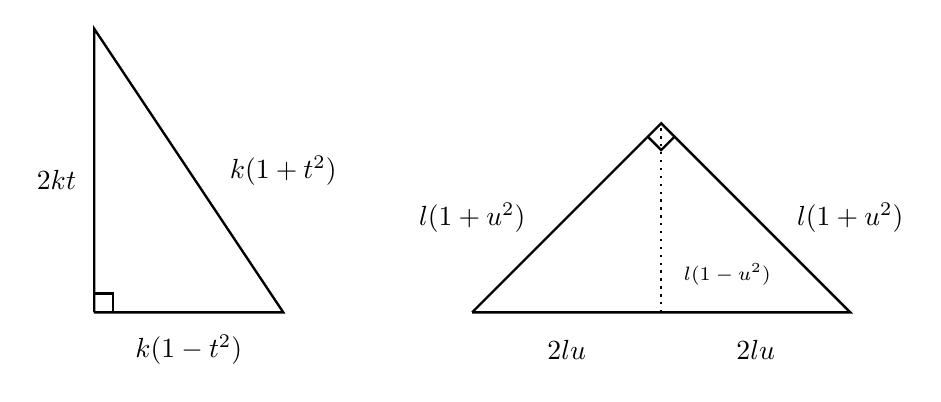
\begin{tikzpicture}[scale=1.2]
	\draw[line width=0.03cm] (0,0) -- (0,3) -- (2,0) -- (0,0);
	\draw[line width=0.03cm] (0,0.2) -- (0.2,0.2) -- (0.2,0);
	\node at (1,-0.4) {$k(1-t^2)$};
	\node at (-0.4,1.4) {$2kt$};
	\node at (2.0,1.5) {$k(1+t^2)$};
	
	\draw[line width=0.03cm] (4,0) -- (6,2) -- (8,0) -- (4,0);
	\draw[line width=0.03cm,dotted] (6,0) -- (6,2);
	\draw[line width=0.03cm] (5.85858,1.85858) -- (6,1.71716) -- (6.14142,1.85858);
	\node at (4,1) {$l(1+u^2)$};
	\node at (8,1) {$l(1+u^2)$};
	\node at (5,-0.4) {$2lu$};
	\node at (7,-0.4) {$2lu$};
	\node at (6.7,0.4) {\scriptsize$l(1-u^2)$};
	\end{tikzpicture}
	\caption{A hypothetical pairing of a rational right triangle and rational isosceles triangle with the same area and perimeter.\label{fig:simtriangles}}
	\end{figure}


Rescaling each triangle by the same factor preserves the equality of the area and the perimeter. Therefore without loss of generality, we may assume that $l= 1$. Equating the areas and perimeters, we find the following simultaneous system of equations:
	\[
	\begin{cases}
	k^2 t (1 - t^2)= 2u (1 - u^2) \\
	k + kt= 1 + 2u + u^2.
	\end{cases}
	\]
Define $x:= u + 1$. Then reframing these equations using $x$, we obtain
	\[
	\begin{cases}
	k^2 t (1 - t^2)= 2x (x - 1) (x - 2) \\
	k(1+t)= x^2.
	\end{cases}
	\]
Writing the first line as $kt(1-t) \cdot k(1+t)$ and solving for $t$ and $1-t$ in the second equation, we can make the substitutions
	\[
	k(1 + t)= x^2, \quad t= \dfrac{x^2 - k}{k}, \quad 1 - t= \dfrac{2k - x^2}{k},
	\]
to obtain the equation
	\[
	x^2 (x^2 - k)(2k - x^2)= 2kx(x - 1)(x - 2).
	\]
Noting that $0 < u < 1$, we know that $x > 0$. Dividing both sides of the equation by $x$, expanding, and writing this equation as a quadratic polynomial in $k$, we see there exists $x \in \Q$, $1 < x < 2$, such that 
	\[
	2xk^2 + (-3x^2 - 2x^2 + 6x - 4)k + x^5= 0. 
	\]
The discriminant of this polynomial in $k$ is a rational square. But then for some $y \in \Q$, we have
	\[
	y^2= (-3x^2 - 2x^2 + 6x - 4)^2 - 4(2x)x^5= x^6 + 12x^5 - 32x^4 + 52x^2 - 48x + 16.
	\]
We can then define a curve $\cC(\Q)$ by
	\[
	\cC \colon \enskip y^2= x^6 + 12x^5 - 32x^4 + 52x^2 - 48x + 16.
	\]
Now $\cC$ is a genus 2 hyperelliptic curve (a higher genus `cousin' to the elliptic curve), and we would like to determine $\cC(\Q)$. By Theorem~\ref{thm:faltings}, we know that the set $\cC(\Q)$ is finite. The Jacobian of $\cC$, $J(\cC)$, has $\rank J(\Q)=1$. Also, the Chabauty-Coleman bound gives $\#\cC(\Q) \leq 10$. However, we have yet to actually find any rational points! In fact, we can find 
	\[
	\{\infty^\pm, (0,\pm 4), (1,\pm 1), (2, \pm 8), (12/11,\pm 868/11^3) \} \subseteq \cC(\Q).
	\]
Therefore, we have completely determined $\cC(\Q)$. Furthermore, the rational point $(12/11,868/11^3)$ gives us a unique pair of such triangles. It was Hirakawa and Matsumura in 2018 that answered this discriminant question (and hence the triangle question), using generalizations of the method of Chabauty, in the affirmative. They show there are exactly one pair of such triangles.


\begin{thm}[{\cite{hirakawamatsumura19}}]
Up to similitude, there exists a unique pair of rational right triangles and a rational isosceles triangle which have the same perimeter and the same area. The unique pair consists of the right triangle with side $(377,135,352)$. and isosceles triangle with sides $(366,366,132)$. 
\end{thm}
\end{ex}